\documentclass[12pt,a4paper]{article}

\usepackage[utf8]{inputenc}
\usepackage[T5]{fontenc}
\usepackage[vietnamese]{babel}
\usepackage{geometry}
\usepackage{graphicx}
\usepackage{amsmath}
\usepackage{booktabs}
\usepackage{array}
\usepackage{float}
\usepackage{xcolor}
\usepackage{hyperref}

\geometry{margin=2.2cm}
\graphicspath{{figures/ai_test_validation/}}
\hypersetup{colorlinks=true, linkcolor=blue, urlcolor=blue}

\title{\textbf{Báo cáo mô hình AI và kết quả kiểm thử}}
\author{AIoT Smart Trash Bin}
\date{Ngày thực hiện: 26/06/2026}

\begin{document}
\maketitle

\section{Tổng quan}
Hệ thống thùng rác thông minh sử dụng mô hình AI để phân biệt hai loại rác
chính: \texttt{paper} và \texttt{plastic}. Kết quả vận hành cuối cùng của hệ
thống gồm ba nhãn:

\begin{center}
\texttt{PAPER}, \texttt{PLASTIC}, \texttt{OTHER}
\end{center}

Trong lần huấn luyện này, mô hình CNN chỉ học hai lớp \texttt{paper} và
\texttt{plastic}. Nhãn \texttt{OTHER} không được train như lớp thứ ba, mà được
tạo bằng cơ chế từ chối dựa trên độ tin cậy, độ chênh xác suất và khoảng cách
embedding tới centroid.

\section{Dữ liệu sử dụng}
Dữ liệu được lấy từ tập TrashNet có sẵn trong thư mục \texttt{AI/trashnet/data}.
Chỉ ảnh \texttt{paper} và \texttt{plastic} được dùng để cập nhật trọng số mô
hình. Các lớp khác như \texttt{cardboard}, \texttt{glass}, \texttt{metal} và
\texttt{trash} chỉ dùng để kiểm tra khả năng từ chối \texttt{OTHER}.

\begin{table}[H]
\centering
\caption{Thống kê dữ liệu}
\begin{tabular}{lrrr}
\toprule
\textbf{Tập dữ liệu} & \textbf{Paper} & \textbf{Plastic} & \textbf{Other} \\
\midrule
Train & 403 & 347 & -- \\
Validation & 83 & 61 & 184 \\
Test & 108 & 74 & 249 \\
\bottomrule
\end{tabular}
\end{table}

\section{Tiền xử lý ảnh}
Pipeline tiền xử lý được thiết kế để giống với pipeline dự kiến trên ESP32-CAM:

\begin{itemize}
    \item Crop vùng trung tâm của ảnh theo dạng hình vuông.
    \item Resize ảnh về kích thước $96 \times 96$.
    \item Chuyển ảnh sang thứ tự kênh RGB.
    \item Chuẩn hóa pixel về khoảng $[0, 1]$ khi train model float.
    \item Khi export INT8, input được lượng tử hóa với scale
    \texttt{0.0039215689} và zero point \texttt{-128}.
\end{itemize}

\section{Mô hình AI sử dụng}
Mô hình được sử dụng là Tiny CNN có các khối convolution nhẹ, phù hợp với hướng
triển khai trên thiết bị nhúng. Kiến trúc ưu tiên Depthwise Separable
Convolution để giảm số tham số và kích thước model.

\begin{table}[H]
\centering
\caption{Kiến trúc Tiny CNN}
\begin{tabular}{>{\raggedright\arraybackslash}p{5cm}
                >{\raggedright\arraybackslash}p{7cm}}
\toprule
\textbf{Thành phần} & \textbf{Mô tả} \\
\midrule
Input & Ảnh RGB kích thước $96 \times 96 \times 3$ \\
Stem convolution & Conv2D $3 \times 3$, 12 filters, stride 2, BatchNorm, ReLU6 \\
Block 1 & DepthwiseConv2D + Pointwise Conv2D 24 filters, BatchNorm, ReLU6 \\
Block 2 & DepthwiseConv2D + Pointwise Conv2D 32 filters, BatchNorm, ReLU6 \\
Block 3 & DepthwiseConv2D + Pointwise Conv2D 48 filters, BatchNorm, ReLU6 \\
Block 4 & DepthwiseConv2D + Pointwise Conv2D 64 filters, BatchNorm, ReLU6 \\
Pooling & Global Average Pooling \\
Embedding & Dense 32, dùng cho tính khoảng cách centroid \\
Output & Dense 2 logits: \texttt{paper}, \texttt{plastic} \\
\bottomrule
\end{tabular}
\end{table}

Số tham số của mô hình là 9,898 tham số. Model deploy xuất hai output:
\texttt{logits} gồm 2 giá trị và \texttt{embedding} gồm 32 chiều. Embedding này
được dùng để hỗ trợ quyết định \texttt{OTHER}.

\section{Cơ chế quyết định OTHER}
Với mỗi ảnh đầu vào, model tạo xác suất cho hai lớp \texttt{paper} và
\texttt{plastic}. Sau đó hệ thống tính:

\begin{itemize}
    \item \textbf{Confidence}: xác suất lớn nhất giữa hai lớp.
    \item \textbf{Margin}: độ chênh giữa xác suất \texttt{paper} và
    \texttt{plastic}.
    \item \textbf{Embedding distance}: khoảng cách từ embedding của ảnh tới
    centroid của lớp được dự đoán.
\end{itemize}

Luật quyết định:
\[
\text{Nếu confidence thấp hoặc margin thấp hoặc distance quá lớn}
\Rightarrow \texttt{OTHER}
\]

Ngưỡng sau calibration hiện tại:

\begin{table}[H]
\centering
\caption{Ngưỡng rejection hiện tại}
\begin{tabular}{lr}
\toprule
\textbf{Tham số} & \textbf{Giá trị} \\
\midrule
\texttt{confidence\_min} & 0.5000 \\
\texttt{margin\_min} & 0.0000 \\
\texttt{paper\_distance\_max} & 6.3018 \\
\texttt{plastic\_distance\_max} & 2.7674 \\
\texttt{use\_embedding\_distance} & true \\
\bottomrule
\end{tabular}
\end{table}

Kết quả calibration ghi nhận \texttt{feasible=false}, nghĩa là chưa tìm được bộ
ngưỡng đồng thời giữ recall \texttt{paper/plastic} trên 85\% và false accept
\texttt{OTHER} dưới 10\%.

\section{Huấn luyện và export}
Mô hình được train bằng TensorFlow/Keras với AdamW, early stopping và checkpoint
theo macro F1 trên validation. Sau đó model được export sang TensorFlow Lite
INT8 để chuẩn bị nhúng vào firmware.

\begin{table}[H]
\centering
\caption{Artifact sau khi train và export}
\begin{tabular}{ll}
\toprule
\textbf{Artifact} & \textbf{Ý nghĩa} \\
\midrule
\texttt{model\_float.keras} & Model float sau train \\
\texttt{model\_int8.tflite} & Model lượng tử hóa INT8 \\
\texttt{model\_data.cc/.h} & Mảng C để nhúng vào firmware ESP32 \\
\texttt{labels.json} & Ánh xạ nhãn paper/plastic \\
\texttt{thresholds.json} & Ngưỡng quyết định OTHER \\
\texttt{centroids.json} & Centroid embedding cho từng lớp \\
\texttt{quantization.json} & Thông tin scale/zero point của INT8 model \\
\texttt{metrics\_int8.json} & Kết quả đánh giá model INT8 \\
\bottomrule
\end{tabular}
\end{table}

Model INT8 có kích thước 25,096 bytes. Input và output đều ở kiểu
\texttt{int8}, phù hợp yêu cầu full integer quantization.

\section{Kết quả kiểm thử hai lớp paper/plastic}
Bảng này chỉ đánh giá khả năng phân biệt hai lớp đã train, chưa tính nhãn
\texttt{OTHER}.

\begin{table}[H]
\centering
\caption{Kết quả kiểm thử paper/plastic}
\begin{tabular}{lrrrr}
\toprule
\textbf{Model} & \textbf{Accuracy} & \textbf{Macro F1} &
\textbf{Recall paper} & \textbf{Recall plastic} \\
\midrule
Tiny CNN float & 87.91\% & 87.53\% & 88.89\% & 86.49\% \\
Tiny CNN INT8 & 87.36\% & 86.99\% & 87.96\% & 86.49\% \\
\bottomrule
\end{tabular}
\end{table}

\begin{figure}[H]
\centering
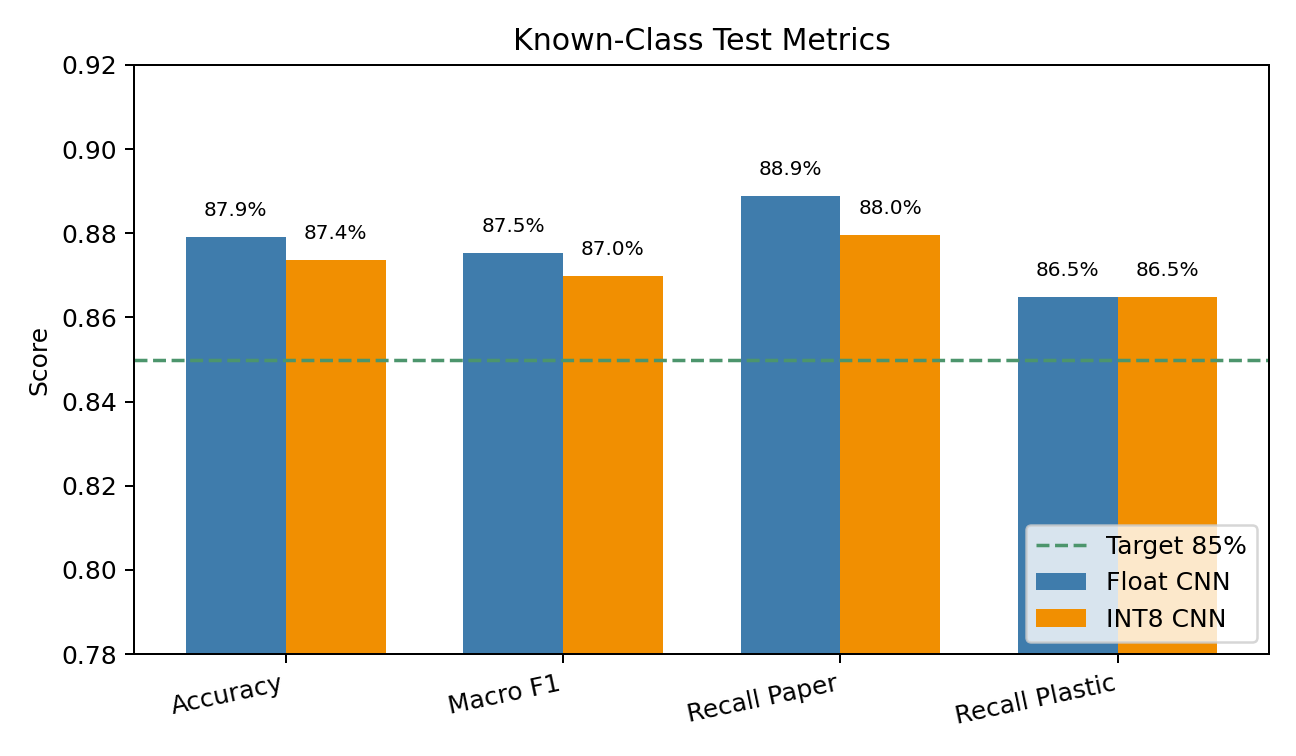
\includegraphics[width=0.92\linewidth]{known_metric_comparison.png}
\caption{So sánh kết quả kiểm thử hai lớp giữa model float và model INT8.}
\end{figure}

Kết quả cho thấy model INT8 giữ chất lượng gần tương đương model float. Accuracy
giảm từ 87.91\% xuống 87.36\%, tức giảm khoảng 0.55 điểm phần trăm.

\section{Kết quả kiểm thử ba đầu ra}
Khi bật cơ chế rejection để tạo nhãn \texttt{OTHER}, kết quả trên tập test ba
đầu ra như sau:

\begin{table}[H]
\centering
\caption{Kết quả kiểm thử ba đầu ra}
\begin{tabular}{lrrrrr}
\toprule
\textbf{Model} & \textbf{Accuracy} & \textbf{Macro F1} &
\textbf{Recall paper} & \textbf{Recall plastic} &
\textbf{Other false accept} \\
\midrule
Tiny CNN float & 39.68\% & 39.18\% & 88.89\% & 82.43\% & 94.38\% \\
Tiny CNN INT8 & 39.68\% & 39.42\% & 87.96\% & 82.43\% & 93.98\% \\
\bottomrule
\end{tabular}
\end{table}

\begin{table}[H]
\centering
\caption{Confusion matrix của model INT8 sau rejection}
\begin{tabular}{lrrr}
\toprule
\textbf{Thực tế / Dự đoán} & \textbf{PAPER} & \textbf{PLASTIC} & \textbf{OTHER} \\
\midrule
PAPER & 95 & 12 & 1 \\
PLASTIC & 10 & 61 & 3 \\
OTHER & 64 & 170 & 15 \\
\bottomrule
\end{tabular}
\end{table}

\begin{figure}[H]
\centering
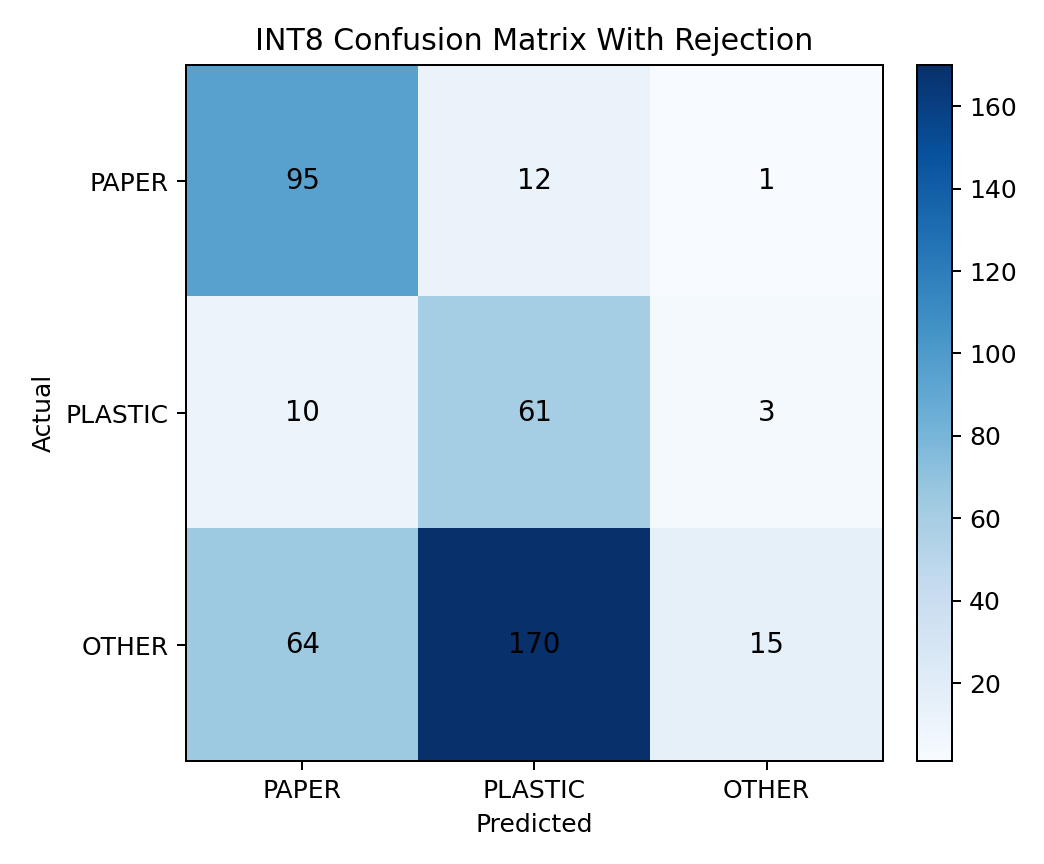
\includegraphics[width=0.72\linewidth]{int8_confusion_matrix.png}
\caption{Confusion matrix của model INT8 khi đánh giá ba đầu ra.}
\end{figure}

\begin{figure}[H]
\centering
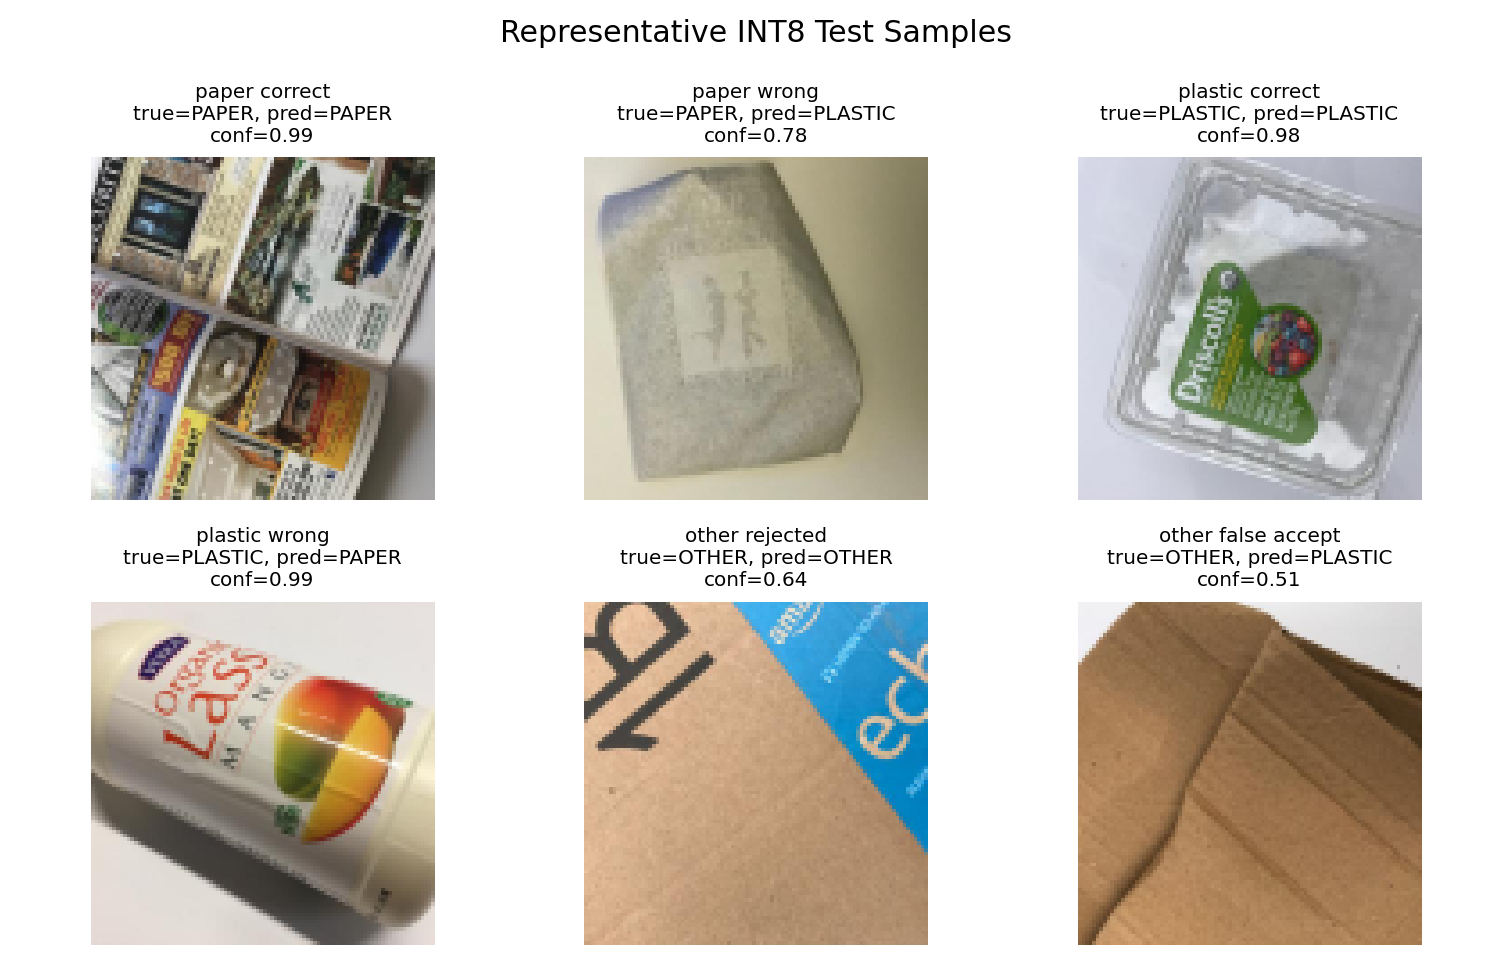
\includegraphics[width=0.95\linewidth]{int8_test_samples.png}
\caption{Một số ảnh minh chứng trong tập test INT8.}
\end{figure}

\section{Nhận xét}
Model Tiny CNN đã cải thiện rõ so với baseline cũ và đạt mục tiêu recall cho
hai lớp chính trên tập test hiện tại. Việc lượng tử hóa INT8 không làm suy giảm
đáng kể chất lượng phân loại \texttt{paper/plastic}.

Tuy nhiên, phần \texttt{OTHER} chưa đạt yêu cầu. Tỷ lệ false accept của
\texttt{OTHER} lên tới 93.98\%, cao hơn nhiều so với mục tiêu không quá 10\%.
Điều này cho thấy các ảnh ngoài hai lớp chính trong TrashNet chưa đủ phù hợp để
calibrate bộ lọc \texttt{OTHER}, hoặc embedding hiện tại chưa tách tốt vật lạ
ra khỏi giấy/nhựa.

\section{Kết luận}
Mô hình AI đang sử dụng là Tiny CNN hai lớp, đầu vào $96 \times 96 \times 3$,
có embedding 32 chiều và được export thành model INT8 kích thước 25,096 bytes.
Model đạt kết quả tốt cho hai lớp \texttt{paper} và \texttt{plastic}, với
accuracy INT8 87.36\% và recall từng lớp đều trên 85\%.

Hệ thống chưa đạt nghiệm thu hoàn chỉnh ba đầu ra vì cơ chế \texttt{OTHER}
chưa ổn định. Bước tiếp theo cần bổ sung dữ liệu \texttt{OTHER} thực tế được
chụp bằng prototype, calibrate lại threshold, sau đó kiểm thử trên ESP32-CAM và
kiểm thử end-to-end với servo.

\end{document}
